\documentclass[border=10pt]{standalone}
\usepackage[svgnames]{xcolor}
\usepackage{amsmath}
\usepackage{pgfplots}
\pgfplotsset{compat=newest}
\usepackage[sfdefault]{FiraSans}
\usepackage{FiraMono}
\renewcommand*\familydefault{\sfdefault}
\begin{document}
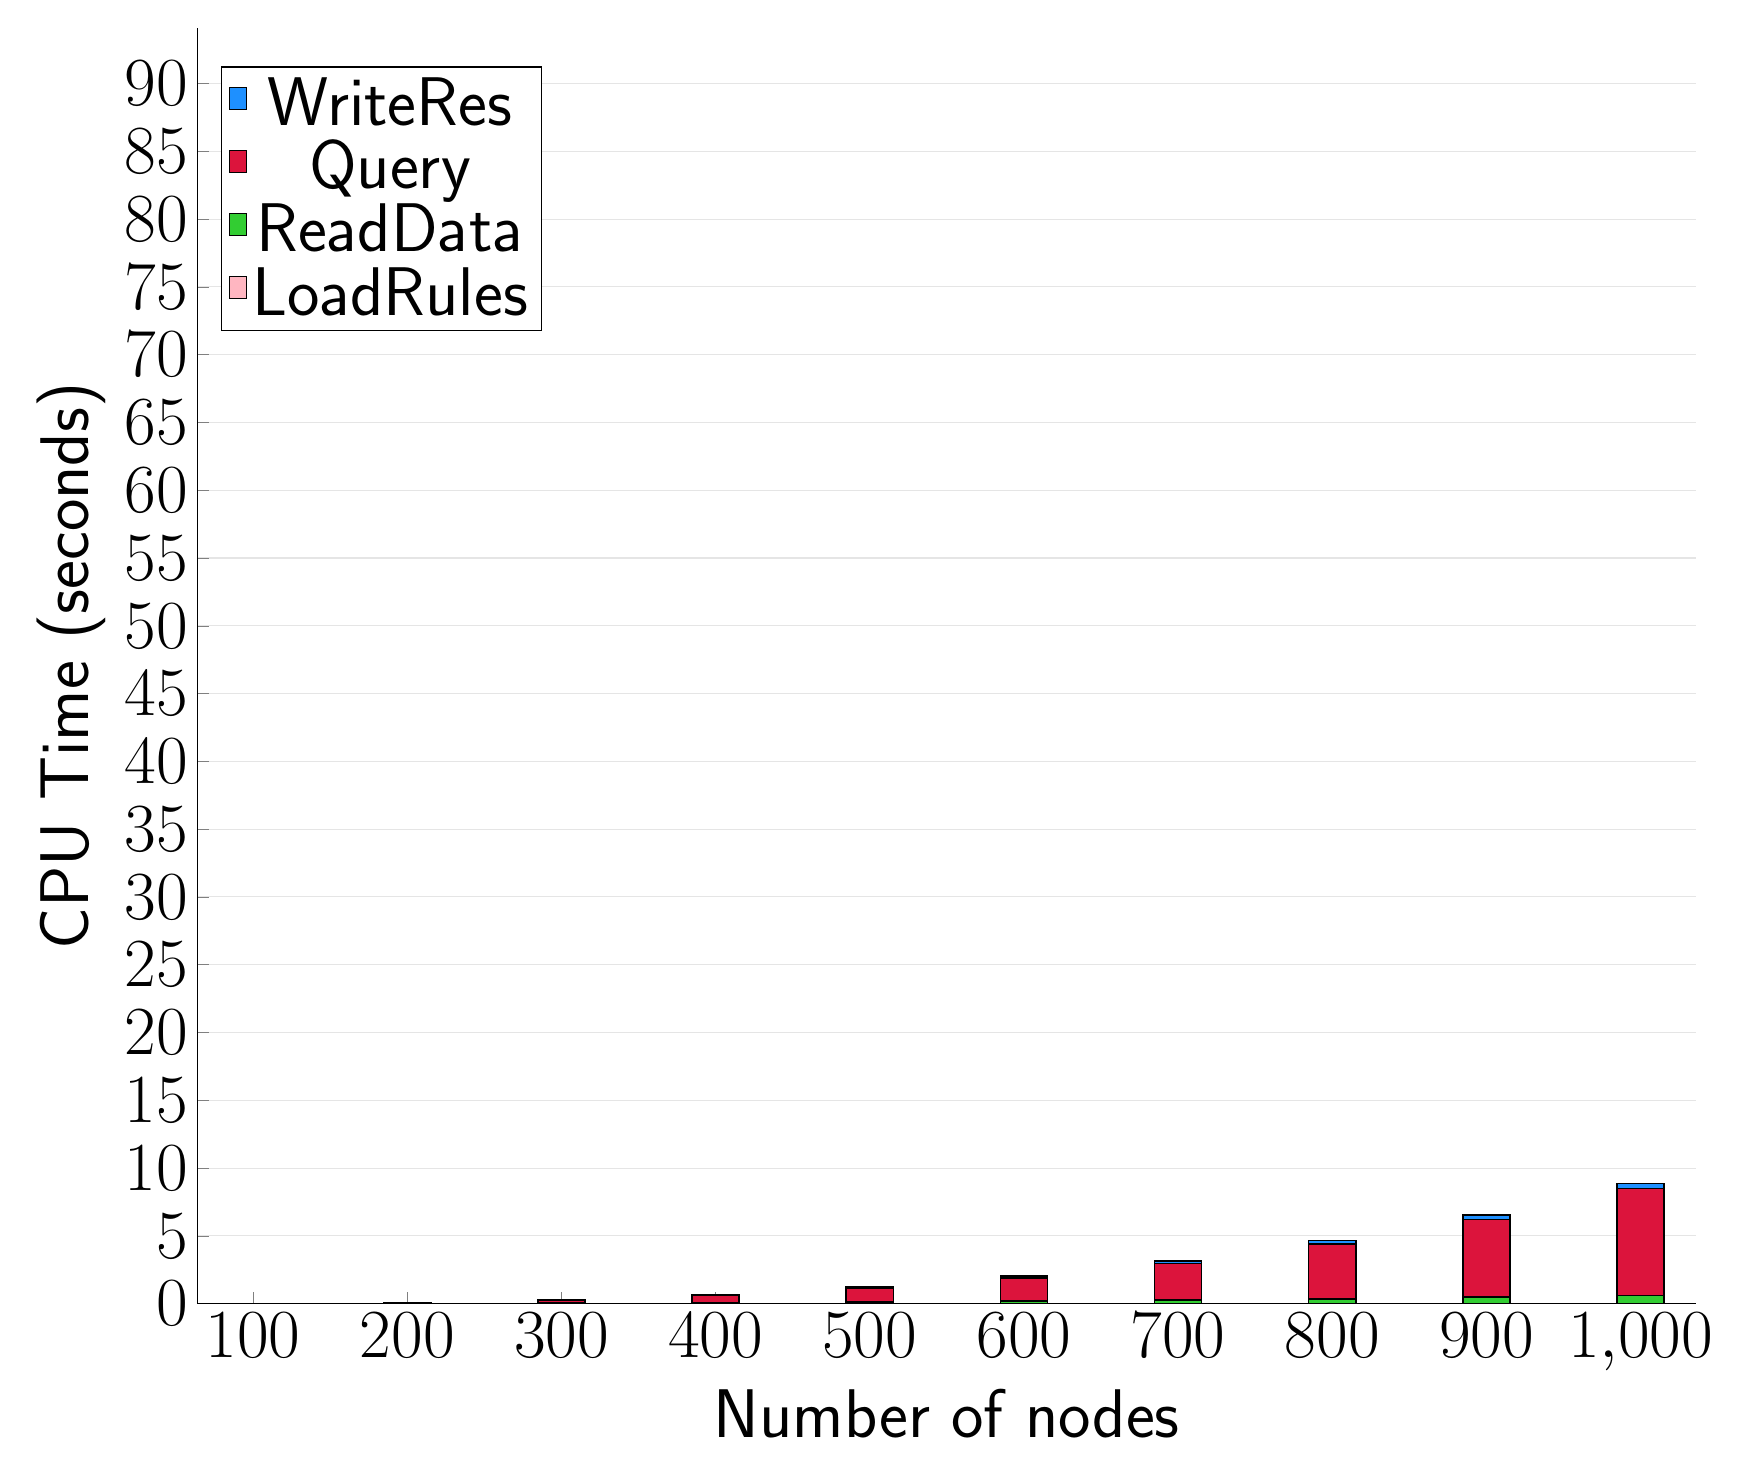
\begin{tikzpicture}
\begin{axis}[
   ybar stacked,
   width=1.7\textwidth,
   bar width=0.6cm,
   ymajorgrids, tick align=inside,
   major grid style={draw=gray!20},
   xtick=data,
   ymin=0, ymax=94.08204,
   axis x line*=bottom,
   axis y line*=left,
   enlarge x limits=0.04,
   legend style={
       at={(0.23, 0.97)},
       anchor=north east,
       legend columns=1,
       font=\Huge,
   },
   ylabel={CPU Time (seconds)},
   xlabel={Number of nodes},
   label style={font=\Huge},
   tick label style={font=\Huge},
]
\addlegendimage{fill=DodgerBlue, draw=black, line width=0.2pt}
\addlegendentry{WriteRes}
\addlegendimage{fill=Crimson, draw=black, line width=0.2pt}
\addlegendentry{Query}
\addlegendimage{fill=LimeGreen, draw=black, line width=0.2pt}
\addlegendentry{ReadData}
\addlegendimage{fill=LightPink, draw=black, line width=0.2pt}
\addlegendentry{LoadRules}
\addplot +[fill=LightPink, draw=black, line width=0.55pt] coordinates {
(100, 0.0005547999999999996)
(200, 0.0005504000000000008)
(300, 0.0005564)
(400, 0.0005506000000000006)
(500, 0.0005567999999999999)
(600, 0.0005564000000000002)
(700, 0.000556)
(800, 0.0005768000000000004)
(900, 0.0005512000000000002)
(1000, 0.0005521999999999998)
};
\addplot +[fill=LimeGreen, draw=black, line width=0.55pt] coordinates {
(100, 0.0040346)
(200, 0.0169738)
(300, 0.0402016)
(400, 0.0752574)
(500, 0.1222176)
(600, 0.1827722)
(700, 0.26026819999999995)
(800, 0.3548876)
(900, 0.4689064)
(1000, 0.6056752)
};
\addplot +[fill=Crimson, draw=black, line width=0.55pt] coordinates {
(100, 0.0081698)
(200, 0.06541759999999999)
(300, 0.21946680000000002)
(400, 0.5156459999999999)
(500, 1.0029584)
(600, 1.7041092)
(700, 2.6984041999999997)
(800, 4.031386599999999)
(900, 5.747338999999999)
(1000, 7.870228)
};
\addplot +[fill=DodgerBlue, draw=black, line width=0.55pt] coordinates {
(100, 0.0039835999999999995)
(200, 0.0162606)
(300, 0.03402940000000001)
(400, 0.06146259999999999)
(500, 0.1020458)
(600, 0.14208860000000004)
(700, 0.18749259999999995)
(800, 0.27180780000000004)
(900, 0.3338723999999999)
(1000, 0.391597)
};
\end{axis}
\end{tikzpicture}

\end{document}
